\begin{frame}
\frametitle{GLOW}
    \begin{itemize}
        \item Flow-based generative model   
        \item Uses invertible 1x1 convolutions 
        \item Builds off of NICE and RealNVP (will leave out redundant info)
        \item Paper has a good overview of generative models and the
        differences.
    \end{itemize}
\end{frame}

\begin{frame}
\frametitle{Model}
\center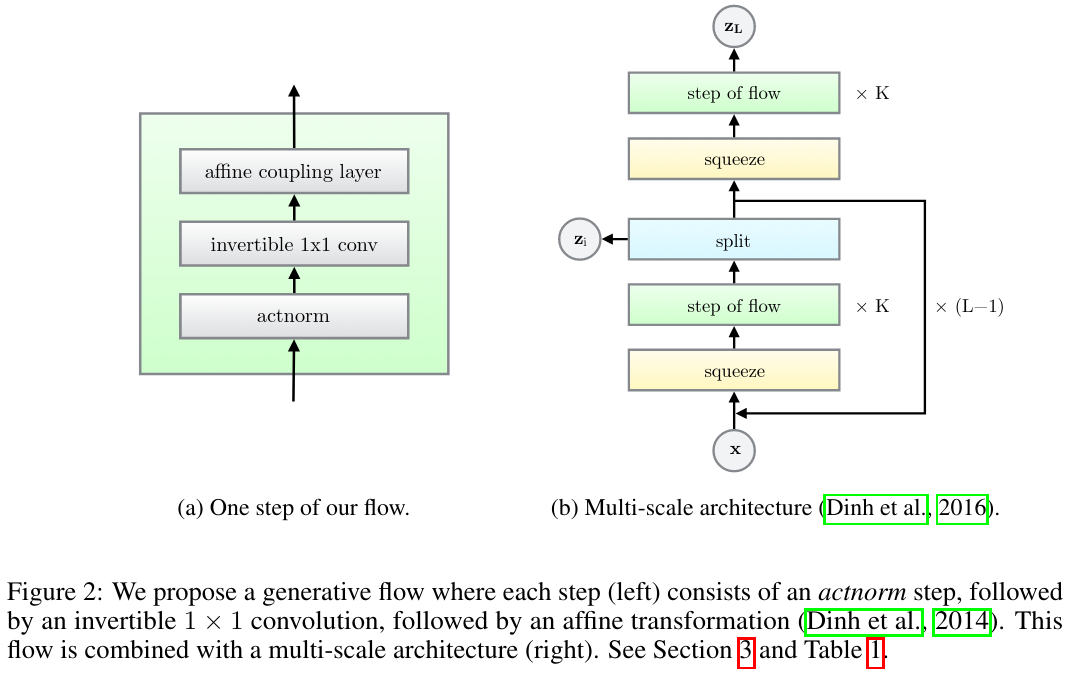
\includegraphics[width=0.8\textwidth]{GLOWModel.png}
\end{frame}

\begin{frame}
\frametitle{Model Components}
\center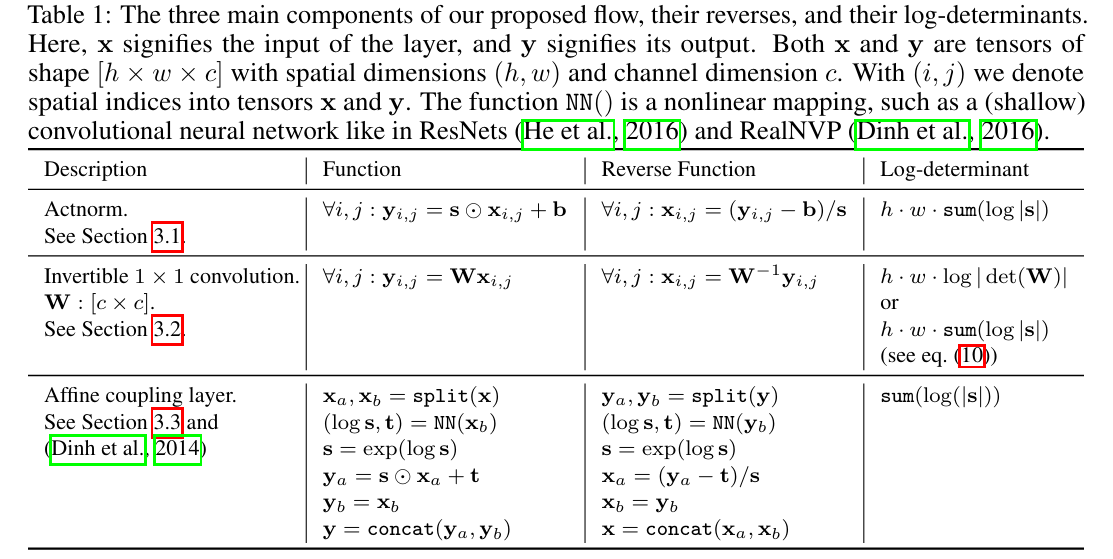
\includegraphics[width=0.8\textwidth]{GLOWComponents.png}
\end{frame}

\begin{frame}
\frametitle{Invertible 1x1 Convolutions}
    \begin{itemize}
        \item NICE uses a flow that uses a reverse permutation for channel ordering.
        \item GLOW learns this permutation with a 1x1 convolution
    \end{itemize}
    \begin{equation}
        log \left| det \left(\frac{d \textrm{conv2D}(\mathbf{h};\mathbf{W})}
                {d\mathbf{h}}\right)\right| = h \cdot w \cdot \log|det(\mathbf{W})| 
    \end{equation}
    \begin{itemize}
        \item Computing $\mathbf{W}$ can be reduced from $O(c^3)$ to $O(c)$ by
        LU Decomposition
    \end{itemize}
    \begin{align*}
        \mathbf{W} &= \mathbf{PL}(\mathbf{U} + diag(\mathbf{s}))\\
        log|det(\mathbf{W})| &= \sum(\log|\mathbf{s}|)
    \end{align*}
\end{frame}

\begin{frame}
\frametitle{Properties}
    \begin{itemize}
        \item Additive coupling layer has $\mathbf{s}=1$ and log-determinant = 0
        \item Zero initialization helps because they act like an identity
        \item Split and concatenation along channel dimension.
        \item Learned Permutation
    \end{itemize}
\end{frame}

\begin{frame}
\frametitle{GLOW Results}
\center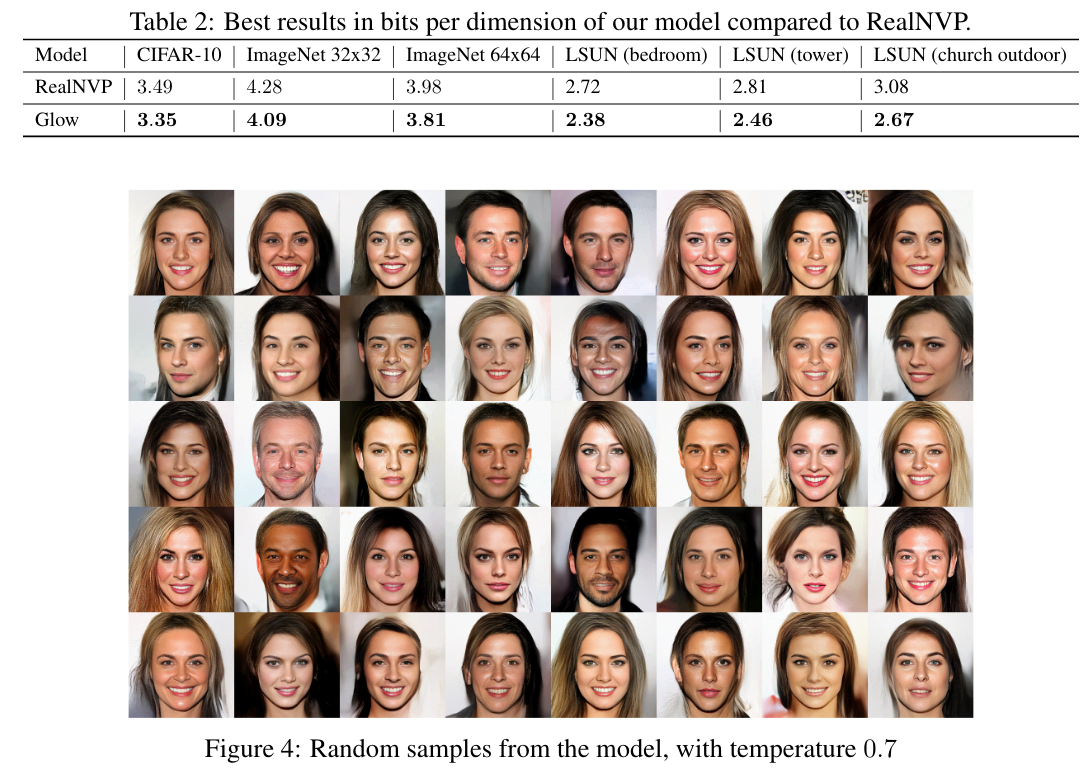
\includegraphics[width=0.8\textwidth]{GLOWResults.png}
\end{frame}
